\section{Zielsetzung}
\label{sec:Ziel}
Ziel des Franck-Hertz-Versuches ist es, das Bohrsche Postulat der diskreten Energieniveaus gebundener Elektronen nachzuweisen.
Zudem lässt sich sowohl die Ionisierungsenergie als auch die Anregungsenergie von Quecksilber bestimmen.

\section{Theorie}
\label{sec:Theorie}

\paragraph{Art der Anregung}
Eine Franck-Hertz-Röhre verwendet durch ein elektro-statisches Feld beschleunigte Elektronen, um beim Stoß dieser mit freien Quecksilberatomen letztere anzuregen. Anregung bedeutet hierbei eines der im Quecksilberatom gebundenen Elektronen auf ein höheres Energieniveau zu bringen, wofür die kinetische Energie $E_{kin} = \frac{1}{2} m_0 v^2$ der Elektronen verwendet wird. Reicht $E_{kin}$ nicht aus ein getroffenes Atom anzuregen, so stoßen Elektron und Atom vollkommen elastisch und durch die große Masse von Quecksilber wird das Elektron lediglich abgelenkt. Kann jedoch eine Anregung stattfinden, so gibt das Elektron die Anregungsenergie $E_A$ an das Atom ab und bewegt sich mit $E_{kin} - E_A$ weiter. Das angeregte Atom gibt dann einen Lichtquant der Energie $E_A=h \nu$ ab, wobei $\nu$ die Frequenz und $h$ das Planck'sche Wirkungsquantum bezeichnet, ab, um in den Grundzustand zurück zu kehren.

\paragraph{Gewinnung und Beschleunigung freier Elektronen}
Die freien Elektronen werden gemäß des Prinzips der Elektronenkanone durch Glühemission gewonnen. Dies bedeutet ein Draht mit hoher Schmelztemperatur und geringer Austrittsarbeit für Elektronen wird stark erhitzt, sodass sich in seinem Umfeld ein Elektronengas mit Energieverteilung $\Delta E$ bildet. Diese nun freien Elektronen werden durch die Beschleunigungsspannung $U_b$ beschleunigt, d.h. sie erhalten die Energie $E_{kin} = e_0 U_b$ mit $e_0$ als Elementarladung.

\paragraph{Quecksilberdampf}
Gemäß der Dampfdruck-Kurve von Quecksilber ergibt sich zu jeder Temperatur $T$ ein Sättigungsdruck $p_{sät}$ des Quecksilberdampfes mit welchem ein Tropfen Quecksilber die Franck-Hertz-Röhre füllt.
Es gilt
\begin{equation}
  \label{eqn:p}
  p_{sät} = 5.5\cdot10^7 \, \textbf{exp} \left( -6876/T \right),
\end{equation}
wenn $p_{sät}$ in $\si{\milli \bar}$ und $T$ in $\si{\kelvin}$ gegeben sind.
Der mittlere freie Weg $\overline{w}$ (in $\si{\centi \meter}$) ergibt sich hierbei zu

\begin{equation}
  \label{eqn:Weg}
  \overline{w} = \frac{0.0029}{p_{sät}}
\end{equation}

wobei $p_{sät}$ in $\si{\milli \bar}$ ausgedrückt ist.

\paragraph{Komposition einer Franck-Hertz-Röhre}
\begin{figure}
  \center
<<<<<<< HEAD
  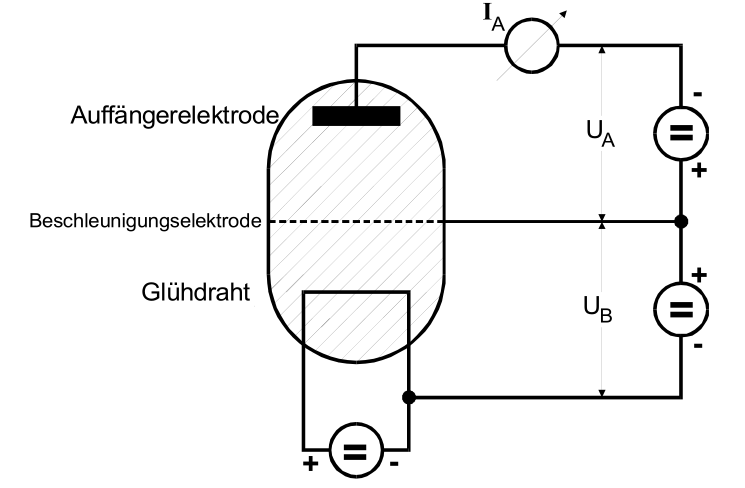
\includegraphics[width=\textwidth]{./logos/roehre.PNG}
||||||| merged common ancestors
  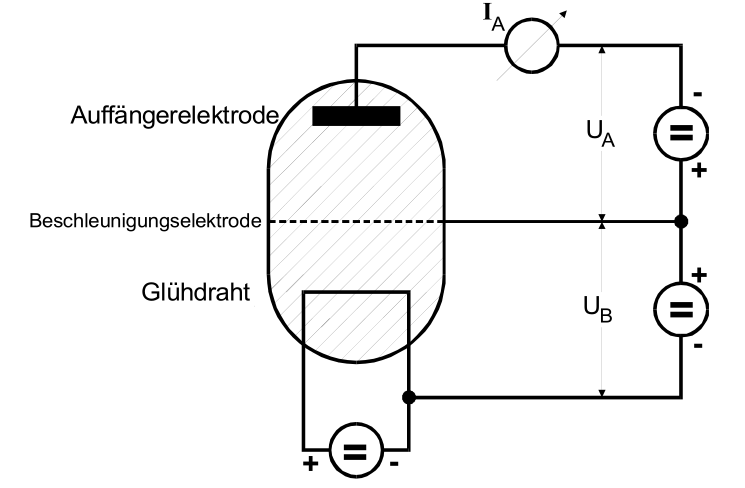
\includegraphics[width=\textwidth]{./logos/roehre.png}
=======
  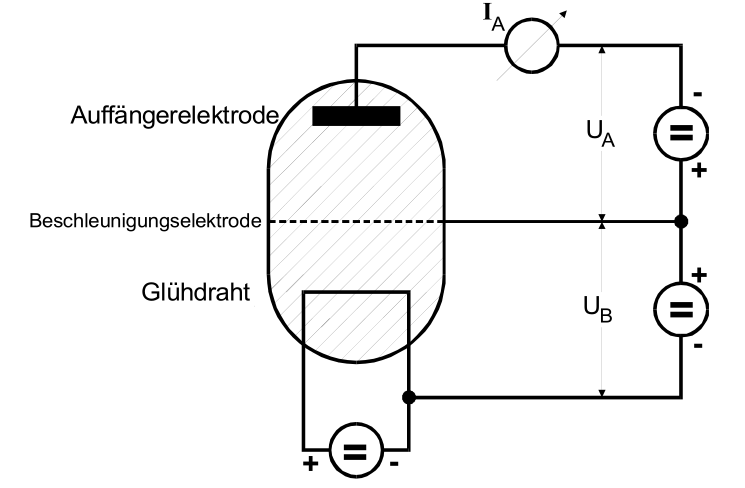
\includegraphics[height = 5cm]{./logos/roehre.png}
>>>>>>> refs/remotes/origin/master
  \caption{Aufbau einer Franck-Hertz-Röhre \cite{Anleitung}}
  \label{fig:roehre}
\end{figure}

Wie in Abb. \ref{fig:roehre} zu erkennen handelt es sich bei der Franck-Hertz-Röhre um ein i.d.R. gläsernes, mit Quecksilberdampf gefülltes Gefäß, dessen drei Kernelemente der Glühdraht, die Gitterelektrode (in der Zeichnung Beschleunigungselektrode genannt), sowie die Auffängerelektrode. Zwischen Glühdraht und Gitterelektrode liegt hierbei die Beschleunigerspannung an, welche die freien Elektronen beschleunigt (abzüglich des Kontaktpotentials $K$ zwischen Glühdraht und Gitterelektrode, bedingt durch unterschiedliche Fermi-Niveaus in den Elektroden) und in den hinter dem Gitter liegenden Bremsbereich einschießt. In diesem vorderen Teil der Röhre finden auch die Stöße statt. Die in diesem Versuchs verwendete Röhre beinhaltet zusätzlich einen variabel steuerbaren Heizdraht zur Temperatur Regelung.

\paragraph{Messung der Elektronenzahl}
Diejenigen Elektronen, welche über eine hinreichende Energie verfügen, um das Bremsfeld zu überwinden, treffen auf der Auffängerelektrode auf, welche über ein hochempfindliches Amperemeter mit der Gitterelektrode verbunden ist. Folglich fließt ein Strom $I_a$ proportional zur Anzahl der auftreffenden Elektronen. Je stärker die Elektronen beschleunigt werden, desto höher ist die Wahrscheinlichkeit, dass Elektronen die Elektrode erreichen. Überschreitet ein Elektron jedoch die Anregungsenergie $E_a$, so gibt es diese Energie beim nächsten Stoß an ein Quecksilberatom ab, d.h. es erreichen schlagartig kaum noch Elektronen den Kollektor, weshalb $I_a$ abfällt. Unter idealisierten Umständen gilt u.a. $\Delta E = 0$, weshalb $I_a$ (instantan) auf 0 fällt. Trägt man nun $I_a$ gegen $U_b$ auf, so erhält man den in Abb. \ref{fig:ideal} dargestellten Zusammenhang.

\begin{figure}
  \center
  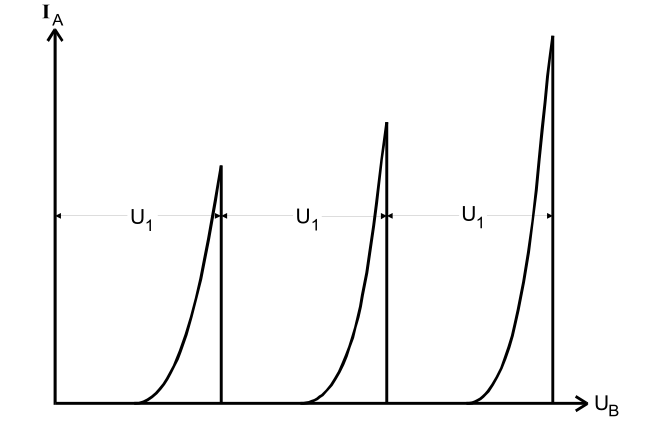
\includegraphics[height = 5cm]{./logos/ideal.PNG}
  \caption{$I_a$ aufgetragen gegen $U_b$ unter Idealbedingungen mit $E_a = e_0 U_1$ \cite{Anleitung}}
  \label{fig:ideal}
\end{figure}
